\subsection{When does DisCo-CFL succeed? Separation and the theory}\label{sec:sep}
\paragraph{Separation predicts success.} Figure~\ref{fig:separation} puts together all 31 scenarios with more than one group, from every benchmark. The estimated separation $\hat\Delta$ and the ARI of DisCo-CFL are strongly associated (Spearman $\rho=0.81$ over scenario means), and the rule ``$\hat\Delta>1-\tau$'' that Theorem~\ref{thm:rec} suggests classifies the scenarios into successes (ARI $\ge0.5$) and failures correctly in 29 of 31 cases, and in 27 of 31 at the stricter recovery level ARI $\ge0.8$ used in the hypotheses of Section~\ref{sec:extra} (there the exceptions are Office-Home, EMNIST label swaps, AG News and the 8-permutation sweep, all with $\hat\Delta>1-\tau$). We give no $p$-value: the scenarios share datasets and models and are not independent, and the association is partly mechanical, because $\hat\Delta$ is computed from the same pooled linkage that the clustering thresholds at $\tau$, which was itself chosen on four of these scenarios. The two exceptions are borderline: the $15^\circ$ rotation ($\hat\Delta=0.06$, ARI $0.52$) and Office-Home ($\hat\Delta=0.13$, ARI $0.26$). EMNIST label swaps, the one scenario where a clearly separated group is split, are counted as a success at ARI $0.56$. The failures of DisCo-CFL are therefore not erratic: they occur where the condition of the theory does not hold. The diagnostic needs the true groups and is computed after the fact; it explains the results but does not choose the reference model in advance (Section~\ref{sec:warmup}).

\begin{figure}[!htbp]
\centering
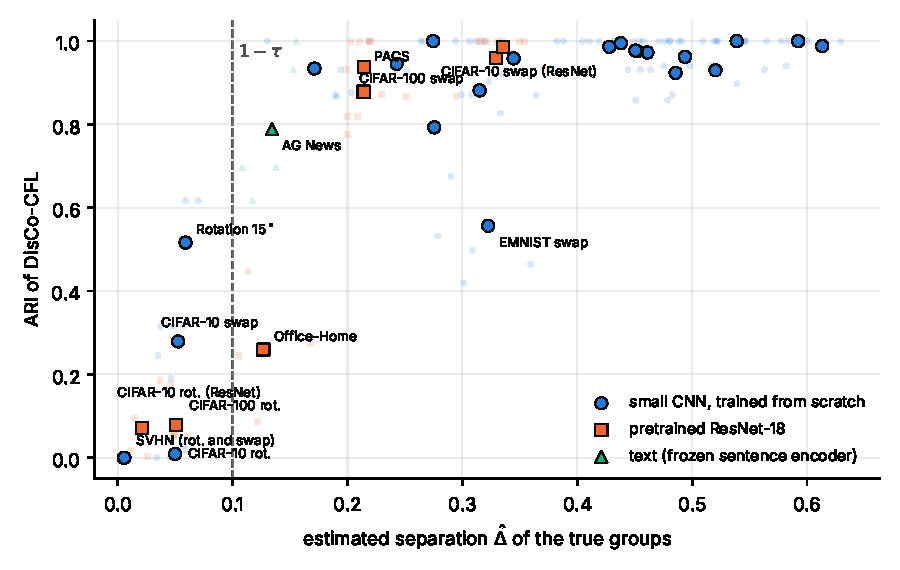
\includegraphics[width=0.85\linewidth]{separation.pdf}
\caption{ARI of DisCo-CFL against the estimated separation $\hat\Delta$ of the true groups, for all 31 scenarios with more than one group (large markers: means over seeds; small markers: individual runs). The dashed line is $1-\tau$, the separation that Theorem~\ref{thm:rec} requires.}\label{fig:separation}
\end{figure}


\paragraph{The results under the shrinkage covered by the theory.} The evidence condition of Theorem~\ref{thm:rec} cannot hold at the default shrinkage $\lambda=0.5$, but it can at $\lambda=0.02$ (Remark~\ref{rem:scope}(e)). We therefore reran the complete pipeline (warm-up, clustering, cluster training and evaluation) with $\lambda=0.02$ on all 24 small-CNN scenarios, with the predictions that accuracy changes by at most $0.5$ points wherever the default recovers the groups and that ARI changes by at most $0.05$ on average (Table~\ref{tab:l02} in Appendix~\ref{app:more}). Both hold. Where the default recovers the groups, mean accuracy changes by $-0.3$ to $+0.2$ points, and over all scenarios the mean absolute change in ARI is $0.014$; the largest changes are on the $15^\circ$ rotation (ARI $0.52\to0.44$) and \emph{Rotation + QS} ($0.99\to0.94$). The classification of the scenarios into successes and failures is the same under the shrinkage that the theorem covers, except for the borderline $15^\circ$ rotation, which falls from ARI $0.52$ to $0.44$; at the stricter level ARI $\ge0.8$, the 8-permutation sweep moves from $0.79$ to $0.81$.

\paragraph{Synthetic signatures.} On synthetic signatures with known ground truth the disattenuated similarity is nearly unbiased, whereas the raw cosine is biased by up to $-0.37$, and the guarantees of Theorem~\ref{thm:rec} are reached once $h\ge64$ (Figure~\ref{fig:theory} in Appendix~\ref{app:more}).
